\hspace{0.5cm} General relativity is an important part of physics which helps us understand our universe in a large scale like black holes, gravitational waves and our expanding universe. It describes gravity as a property of space and time rather than a force as mentioned by Newton. It tells us that the curvature of space-time is related to energy and momentum which is present inside matter. The wrapping of space-time as described by Einstein's field equations theorizes various phenomenons such as gravitational waves. It helps us to understand the region of space having black holes or neutron stars, or system of dynamical heavy masses which causes great changes in gravity.\\ We know that there are three dimensions of space which we can interact with. But Einstein include a fourth dimension namely time. The space-time consists of four dimensional space with three spatial dimensions and a time dimension. In a space, with no matter, the space-time is flat, i.e shortest distance between two points is a straight line, but in presence of matter, shape(curvature) of space-time will be altered, then shortest distance between two points will be a curved line like an hyperbola. It kind of produces a dent in the curvature of space-time. 

\begin{figure}[h]
    \centering
    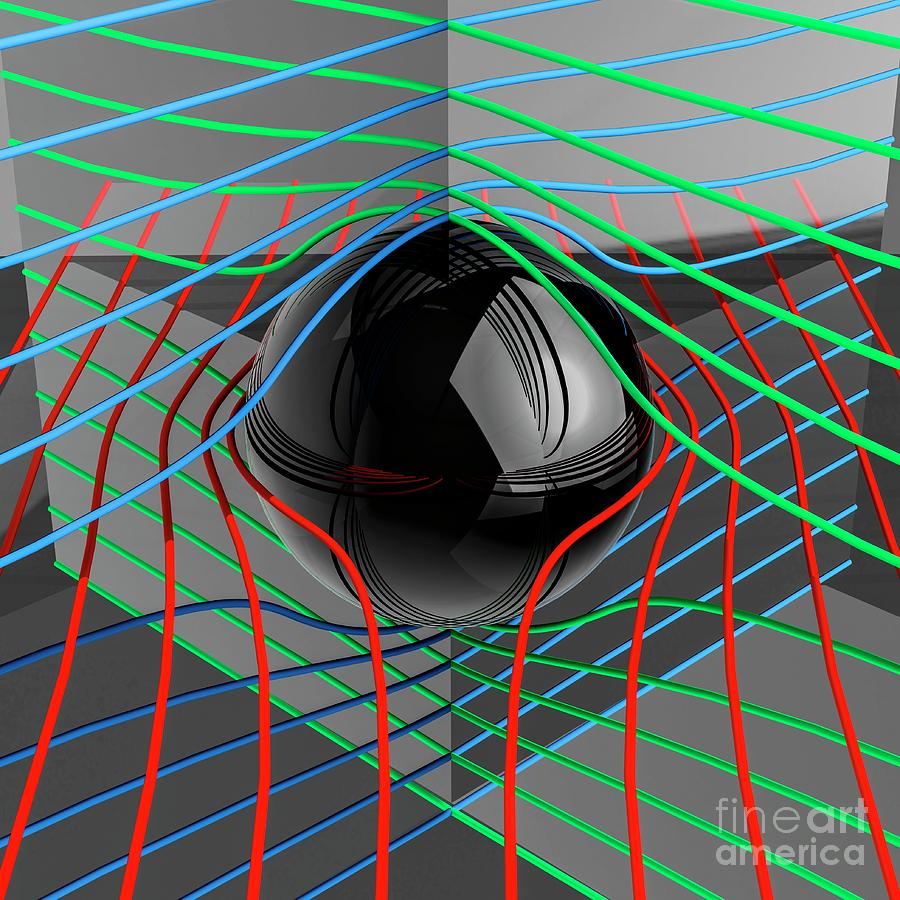
\includegraphics[scale=0.2]{images.tex/illus_3dspace1.jpg}
    \caption{Curved space-time in presence of mass. Source:- \href{https://www.forbes.com/sites/startswithabang/2019/02/16/ask-ethan-how-can-we-measure-the-curvature-of-gravity/?sh=13c20ec1134f}{Forbes.com}}
\end{figure}

If there are two giant masses orbiting around each other, then it results into the formation of ripples in space-time which we call it as gravitational waves. The ripples move with the speed of light. As they move in the space, the farther they move away from the source or their origin, the more weak the get. Their strength decreases as they go away from the source. The gravitational waves which are detected are weak due to various reasons, but are good source of information.\\ In 1916, Einstein predicted that two bodies orbiting each other would not be in the same orbit all the time, instead the bodies lose energy and in doing so emit gravitational waves. According to his mathematics he showed that two massive accelerating objects such as neutron stars or black holes, when orbit around each other, it generates ripples and disrupt the space time such that waves are propagated in all the direction away from the source. This ripples carry the information about their origin and about gravity as well. The strongest gravitational waves are generated due to colliding black holes or neutron star. After half a century, the first indirect proof of gravitational waves was given in the year 1974 when the astronomers Jocelyn Bell and Antony Hewish discovered a pulsar which produces a gravitational wave. After this they were observing how the stars change its orbit as the time passes. They observed that the stars are getting closer to each other at the rate which was predicted by Einstein in his General Relativity which results into production of GW.\\ On September 14, 2015, LIGO sensed a signal which was due to the collision of two massive black holes which are 1.3 billion light years away from Earth. Later after analyzing the phenomena, it was observed that the wave was caused due to objects 29 and 36 times massive than the sun orbiting with 210 kilometer around each other before the collided. The gravitational waves which are generated near the source are very large but by the time they were detected here on earth, their strength was so small that the effect of GW on the detector was 1000 times smaller than the nucleus of an atom.

\pagebreak

